\section{Description des connections}\label{sec:DescConnect}
L'ensemble de l'étage d'alimentation et de commande sont placés dans un boitier électrique qui se branche sur une prise classique 230V. Ce dernier
devra alimenter le contrôleur EPOS4 Compact de chez Maxon \cite{Maxon} et la carte Raspberry Pi \cite{RaspberryPi}. Une tension continue de 48V
sera nécessaire pour commander le moteur et une tension continue de 5V aussi pour alimenter le Raspberry Pi et comme tension logique 1. Pour obtenir
ces tensions, un convertisseur AC-DC avec 48V en sortie et un convertisseur DC-DC avec 48V en entrée et 5V en sortie seront nécessaire. La fiche 230V
sera une fiche pour appareil C14 avec bouton et fusible intégré ce qui enlève la nécessité de mettr un disjoncteur et fait gagner de la place. Les deux
convertisseurs, le contrôleur et la carte de commande sont tous fixés sur un rail DIN35. Il faut donc déterminer les dimensions de ces éléments pour
déterminer la taille du boîtier et du rail nécessaire.\\

Le contrôleur est aussi connecté aux encodeurs linéaire et angulaire, à l'anneau de LEDs et aux capteurs de fin de course. On peut résumer toutes
ces connections sur le schéma suivant.

\begin{figure}[H]
    \centering
    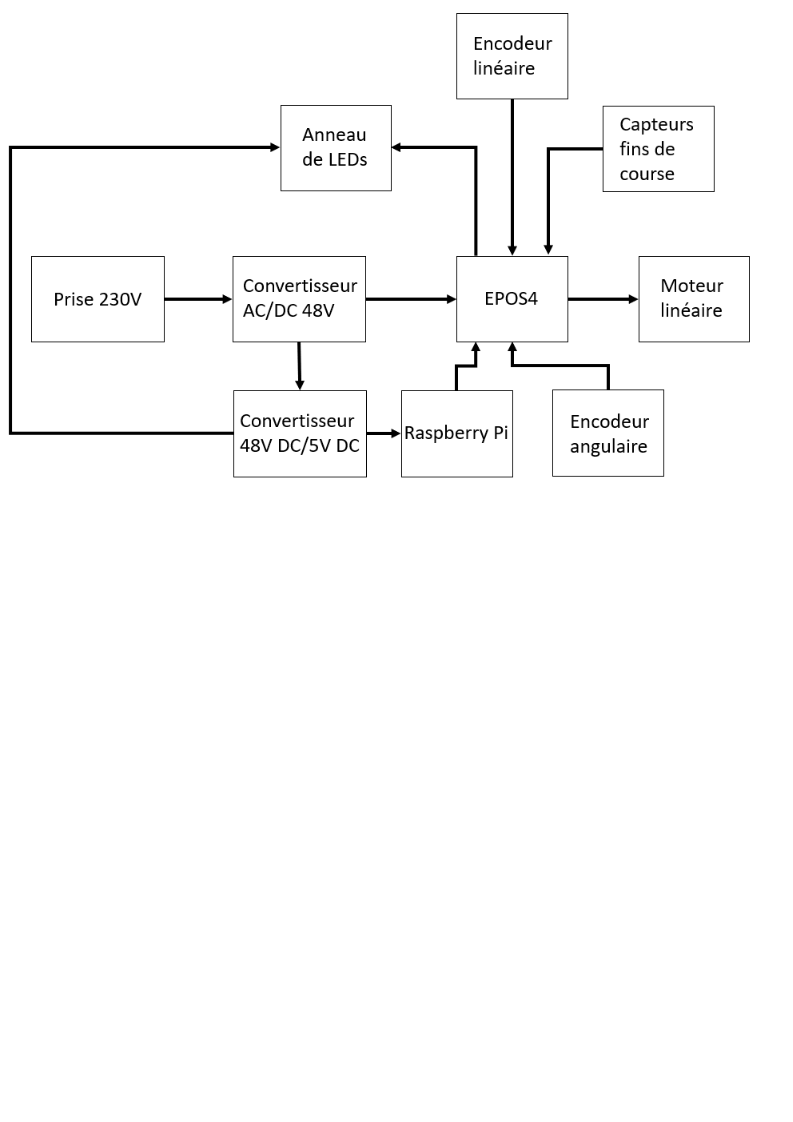
\includegraphics[width = 0.9\textwidth]{assets/figures/SchemaLogique.png}
    \caption{Schéma de connections}
    \label{fig:SchemaConnec}
\end{figure}

\section{Choix des éléments}\label{sec:ChoixElem}

\begin{table}[H]
    \centering
    \caption{Éléments choisis pour le boîtier électrique}
    \label{tab:ChoixElem}
    \resizebox{\textwidth}{!}{%
        \begin{tabular}{|l|l|l|l|l|l|}
            \hline
            Élément                    & Choix               & Fabricant                       & Hauteur {[}mm{]} & Largeur {[}mm{]} & Profondeur {[}mm{]} \\ \hline
            Convertisseur AC-DC 48V    & DRC100US48          & XP Power \cite{XPPower}         & 93               & 70               & 58                  \\ \hline
            Convertisseur DC-DC 48V-5V & DDR-15L-5           & MEAN WELL \cite{MEANWELL}       & 90               & 17.5             & 54.5                \\ \hline
            Contrôleur moteur          & EPOS4 Compact 50/15 & Maxon \cite{Maxon}              & 65.5             & 59.5             & 35                  \\ \hline
            Carte de commande          & Raspberry Pi 4      & Raspberry Pi \cite{RaspberryPi} & 85               & 56               & -                   \\ \hline
            Connecteur fiche 230V      & C14                 & Schurter \cite{Schurter}        & -                & -                & -                   \\ \hline
            Bouton arrêt d'urgence     & AB6E-3BV02PTRH      & IDEC \cite{IDEC}                & -                & -                & -                   \\ \hline
            Bouton poussoir            & 82-5151.1134.B001   & EAO \cite{EAO}                  & -                & -                & -                   \\ \hline
        \end{tabular}%
    }
\end{table}

La somme des largeurs des éléments est de 203~mm, la hauteur la plus grande est de 93~mm et la profondeur la plus élevée est de 58~mm. Le choix
du boîtier se porte sur l'ABS 200/100 HG ENCLOSURE de chez Fibox \cite{Fibox} avec 171~mm de hauteur interne, 95~mm de profondeur interne et
246~mm de largeur interne. Avec il y aussi la plaque de montage MIV 200 MOUNTING PLATE et le rail MIV 20 DIN-35 RAIL aussi de chez Fibox \cite{Fibox}.
L'assemblage de ces pièces ressemble à ceci.

\begin{figure}[H]
    \centering
    \includegraphics[width = 0.8\textwidth]{assets/figures/AssemblageBoitierElectrique.png}
    \caption{Boîtier électrique avec composants}
    \label{fig:AssBoitierElec}
\end{figure}